\chapter{Ausblick}\label{ch:ausblick}
Je weiter sich das Projekt der vorliegenden Arbeit dem Abschluss näherte, desto mehr kristallisierte sich ein Hauptproblem für den praktischen Einsatz heraus.
Das erstellte Template ist sehr auf die DATEV-Rechnungsschreibung spezialisiert, das heißt es ist funktionsfähig, kann aber nicht ohne zeitaufwändige Eingriffe in das Template, in die Workflowdefinitionsdateien und die eigentlichen REXX Skripte und Jobs, an eine andere Anwendung angepasst werden. 
Folglich müsste das Template dynamischer implementiert sein.
Um dies zu verdeutlichen, wird als Beispiel die Provisionierung von IBM MQ Queues herangezogen.
Momentan werden die Prozesse und die Trigger Queues statisch angelegt.
Das heißt, dass sowohl Namen, als auch die damit verknüpften Queueparameter, fest hinterlegt sind, um nur ein Beispiel zu nennen.
Besser wäre es, alle Parameter in der Eingabedatei des Templates anzugeben.
Aus IBM MQ Sicht ist hinzuzufügen, dass die fehlende automatisierte Bereitstellung eines Queue Managers den gewünschten Effekt einer weitgehenden Automatisierung und Unabhängigkeit von der Administration, abschwächt.

Während der Realisierung stellte sich ebenfalls heraus, dass ein Template, das mehrere Subsysteme beinhaltet und dadurch sehr anwendungsspezifisch ist, nicht für einen firmenweiten Einsatz geeignet ist.
So ist zu empfehlen, dass für jedes Subsystem, also CICS, Db2 und IBM MQ, ein separates \glqq Basis\grqq-Template realisiert wird.

Angenommen es besteht für jedes Subsystem ein Template und das IBM MQ Template beinhaltet die Provisionierung eines Queue Managers, so könnte jeder Entwickler seine eigenen Instanzen der Templates besitzen und für eigene Tests nutzen.
Dennoch wäre der ermöglichte Bereitstellungsprozess nicht optimal.
So müsste für jede kleine Änderung an der Konfigurationsdatei ein neues Template erzeugt werden, siehe zweiter Use-Case im Abschnitt \ref{ssec:akttemp2fall}.
Das dort genannte Beispiel einer CICS-Instanz und der notwendigen eindeutigen Application ID wird hier aufgegriffen.
Eine Möglichkeit dieses Problem zu lösen, wäre einen Pool mit verfügbaren Application IDs bereitzustellen und dann mittels eines Programms eine ungenutzte Application ID zu ermitteln.
Dieses Programm könnte dann als Step in das Template aufgenommen werden.
Jedoch müsste immer noch für jede Änderung an der Konfigurationsdatei ein neues Template erzeugt werden.

Hier schafft z/OSPT Abhilfe.
Damit kann, wie in Absatz \ref{sssec:zospt} beschrieben, mit Hilfe der z/OSPT-Datei und dem Konzept der Images das Template von außen konfiguriert werden.
Dadurch fällt das Kopieren des Templates für den Mitarbeiter weg, dieser kann mittels des Kommandozeileninterfaces ein z/OSPT-Image bauen und daraus einen z/OSPT-Container erzeugen.
Das Kommandozeileninterface hat einen weiteren Vorteil.
Mit dessen Hilfe können Arbeitsschritte für die Provisionierung der Middleware über groovy in einen Jenkins-Ablauf aufgenommen werden.
Somit läuft der Prozess automatisiert ab und nähert sich modernen Entwicklungsabläufen wie denen aus der Cloud Native Entwicklung an.

Angenommen es existieren jeweils ein CICS, ein Db2 und ein IBM MQ Template, und diese sind so realisiert, dass sie firmenweit eingesetzt werden können.
Dann wäre der nächste Schritt, die Aufnahme in den \glqq DATEV Marktplatz\grqq, möglich.
Der \glqq DATEV Marktplatz\grqq{} ist eine Weboberfläche, mit der sich Entwicklerteams ihre benötigte PaaS-Umgebung konfigurieren können.
Heute stehen ihnen dort Dienste wie MongoDB, PostgreSQL, Kafka und viele weitere zur Verfügung.
In Zukunft könnten hier auch Dienste wie CICS, Db2 und IBM MQ zur Auswahl stehen.
Dabei ist in Betracht zu ziehen, ob für den User nur bestimmte vorgefertigte Profile, wie \glqq klein\grqq, \glqq mittel\grqq{} und \glqq groß\grqq, auswählbar sind. 
Dies ist in public Clouds bzw. auch bei der DATEV PaaS Lösung ein übliches Vorgehen.
Die im Hintergrund verbundenen Templates und Images müssten dahingehend angepasst werden.
Um einen solchen \glqq Service Broker\grqq{} zu verwirklichen, könnte die von z/OSMF zur Verfügung gestellte REST-API verwendet werden.
Diese ermöglicht den Zugriff auf fast alle z/OSMF Funktionalitäten mittels Http-Requests.
Für die Tenant Zuweisung zu einem Template würde weiterhin die z/OSMF Oberfläche benötigt werden.
Insgesamt ist zu erkennen, dass mit z/OSMF beziehungsweise IBM hier noch Verbesserungen machbar sind.

Diese technische Umsetzung ermöglicht in Zukunft den in Diagramm \ref{fig:proneu} dargestellten Bereitstellungsprozess.
Es ist zu erkennen, dass Verantwortung für die Bereitstellung einer Laufzeitumgebung in der Entwicklungsstage von den Administratorenteams an die Entwicklerteams übertragen wird.
Dadurch wird Kommunikationsaufwand eingespart und einem Entwickler steht binnen weniger Minuten eine funktionsfähige Laufzeitumgebung in der Entwicklungsstage für seine legacy z/OS Anwendung zur Verfügung.
Bei Problemen oder Beratungswunsch unterstützen die Administratorenteams weiterhin.
Der Hauptaufwand der Umsetzung dieser Lösung liegt bei den Administratorenteams.
Der Effizienzgewinn stellt sich ein, wenn für die wichtigsten Anwendungen Templates existieren, die von den Entwicklern jederzeit genutzt werden können, um in isolierten, individuellen Umgebungen zu entwickeln und zu testen.

\begin{figure}[ht!]
\centering
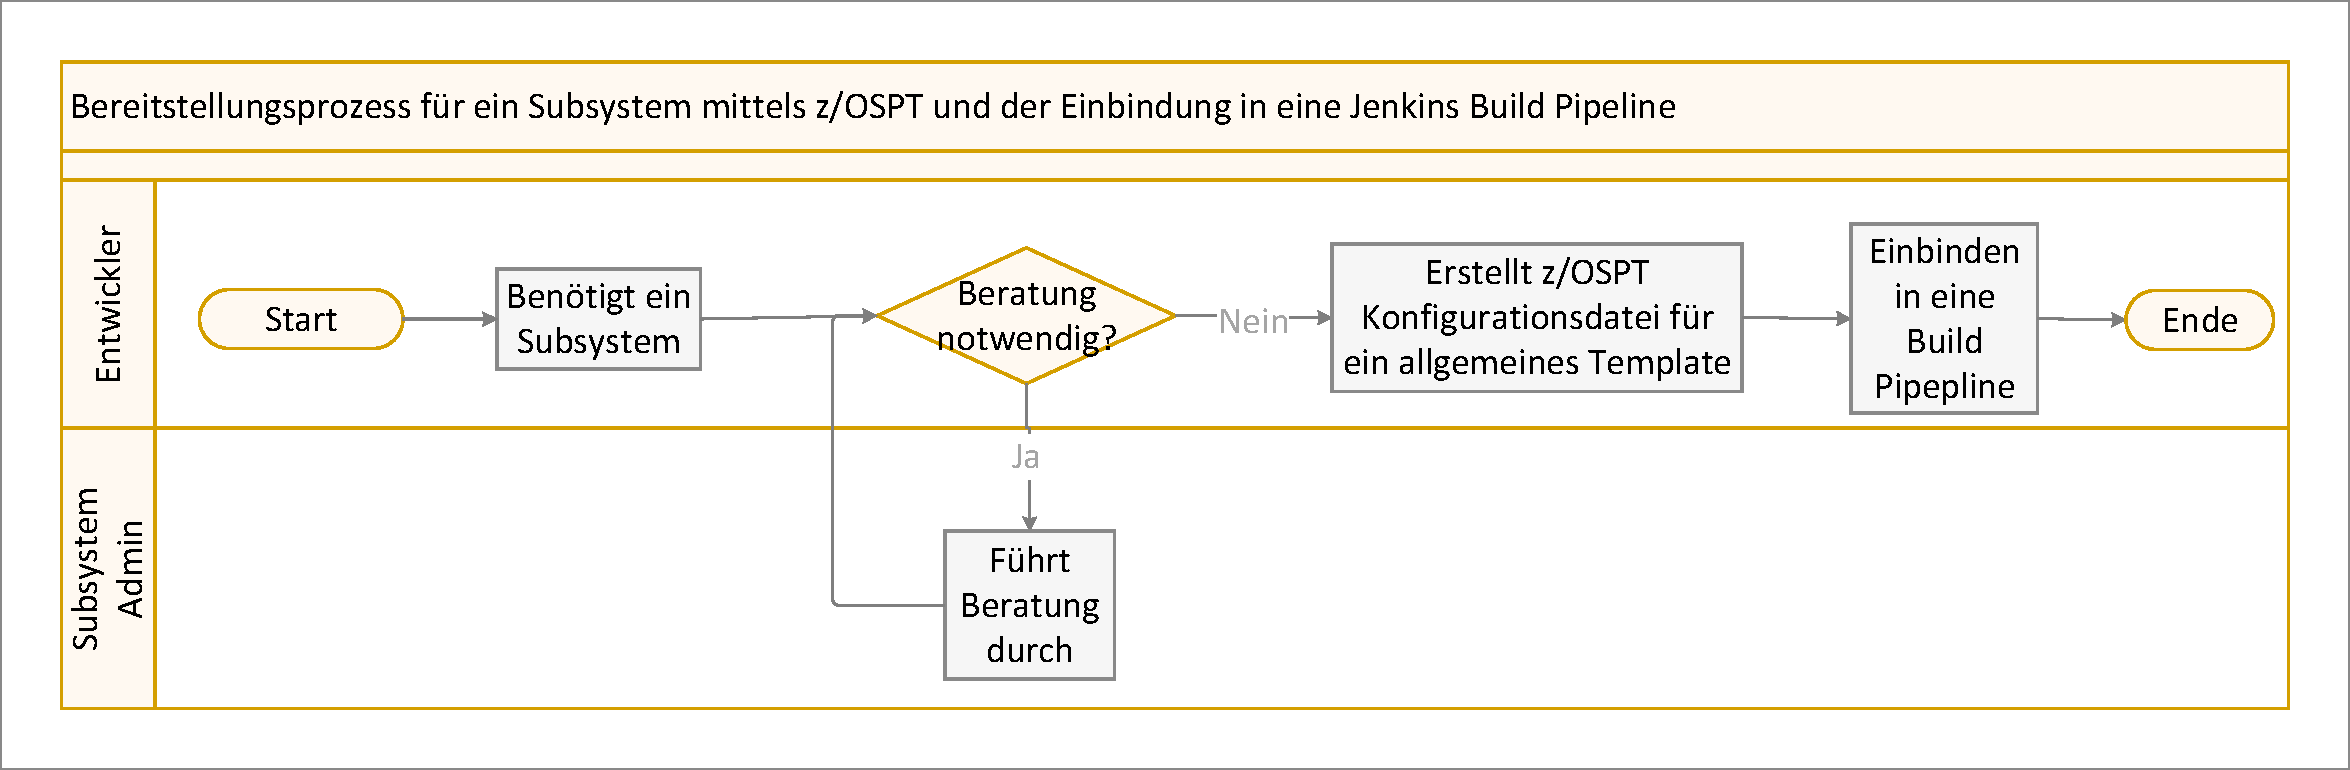
\includegraphics[width=\paperwidth,angle=90]{figures/swimlaneNeuerProzess.pdf}
\caption{Bereistellungsprozess eines Subsystems mittels einer z/OSPT Konfigurationsdatei}
\label{fig:proneu}
\end{figure}

Ist all dies umgesetzt, kann in einem nächsten Schritt der cloud native Aspekt des automatisierten Deployments einer Anwendung inklusive Laufzeitumgebung zwischen Stages bis hin zur Produktion auch für z/OS Anwendungen in Betracht gezogen werden.
